% ----------------------------------------------------------------
% Thesis - Main document
% ----------------------------------------------------------------

\documentclass{thesisclass}
% as defined in thesisclass.cls


%% ---------------------------------
%% | Information about the thesis  |
%% ---------------------------------

\newcommand{\myname}{Jingjian Wei}
\newcommand{\mytitle}{Adversarial Attacks and Defenses for Point Cloud based 3D Object Detection Network}

\newcommand{\reviewerone}{Prof. Dr.-Ing. Christoph Stiller}
\newcommand{\advisor}{Juncong Fei, M.Sc., Ahmed Hammam, M.Sc.}

\newcommand{\timeandplace}{Karlsruhe, Mai 2021}

\newcommand{\frontmatterhint}{Draft! / Vorl\"aufige Fassung!}

%% -------------------------------
%% |  Information for PDF file   |
%% -------------------------------
\hypersetup{
 pdfauthor={\myname},
 pdftitle={\mytitle},
 pdfsubject={Thesis},
 pdfkeywords={}
}
\usepackage[english]{babel}  	% English
%\usepackage[ngerman]{babel}  	% German


%% -------------------------------
%% |    My packages /commands    |
%% -------------------------------
% track changes
    %\usepackage{changes} 		% highlight changes
	\usepackage[final]{changes}	% don't highlight changes

% tables
	\usepackage{array,multirow,graphicx}

% pseudocode
	\usepackage[ruled,vlined]{algorithm2e}

% for forcing positions of tables, figures, ...
	\usepackage{float}

% units
	\usepackage{siunitx}
	\usepackage{dcolumn}
%latex special character
    \usepackage{latexsym}

%% --------------------------------
%% |      glossaries               |
%% --------------------------------
\newif\ifuseglossaries			% as the glossaries package sometimes causes problems, you can switch if of
								% if switching of, remember to remove all \gls{}/... statements
								
\useglossariestrue				% use glossaries (acronyms and online references)
%\useglossariesfalse			% don't use glossaries

\ifuseglossaries
	\usepackage[acronym,xindy,toc,nomain,nonumberlist,nopostdot,notranslate]{glossaries}%

	\newglossary[onlineref]{onlineref}{onli}{onlo}{Online References}
	
	\newglossarystyle{mylong}{%
  		\setglossarystyle{long}%
  		\renewcommand*{\glsnamefont}[1]{\textbf{##1}}%
  	}%
  	
  	\newglossarystyle{mylist}{%
  		\setglossarystyle{list}%
  		\renewcommand*{\glsnamefont}[1]{\textrm{\textmd{##1}}}%
  	}%
  	
  	\makeglossaries
  	
	% ordinary acronyms
	\newacronym{ma}{MA}{My Acronym}
	\newacronym{}{}{}
	% usage: \gls{} \glspl{} or \acrshort{}
	
	% online references
	\newglossaryentry{online_reference}{
		type=onlineref, 
		name={[01]}, 
		description={\hspace{1.5mm}My Online Reference\newline 
			\href{http://www.mrt.kit.edu/}{http://www.mrt.kit.edu/}\newline 
			retrieved 2016-04-28 }}
\else
\fi


%% ---------------------------------
%% | ToDo Marker - only for draft! |
%% ---------------------------------
% Remove this section for final version!
\setlength{\marginparwidth}{20mm}

\newcommand{\margtodo}
{\marginpar{\textbf{\textcolor{blue}{ToDo1}}}{}}


\newcommand{\margmajortodo}
{\marginpar{\textbf{\textcolor{red}{ToDo2}}}{}}

\newcommand{\majortodo}[1]
{{\textbf{\textcolor{red}{(\margmajortodo{}#1)}}}{}}

%% --------------------------------
%% | Draft Marker - only for draft! |
%% --------------------------------
% Remove this section for final version!
%\usepackage{draftwatermark}
%\SetWatermarkText{\hspace{10pt}-draft-}
%\SetWatermarkScale{2.3}
%\SetWatermarkColor[gray]{0.95}


%% --------------------------------
%% | Old Marker - only for draft! |
%% --------------------------------
% Remove this section for final version!
\newenvironment{deprecated}
{\begin{color}{gray}}
{\end{color}}


%% --------------------------------
%% | Settings for word separation |
%% --------------------------------
% Help for separation:
% In german package the following hints are additionally available:
% "- = Additional separation
% "| = Suppress ligation and possible separation (e.g. Schaf"|fell)
% "~ = Hyphenation without separation (e.g. bergauf und "~ab)
% "= = Hyphenation with separation before and after
% "" = Separation without a hyphenation (e.g. und/""oder)

% Describe separation hints here:
\hyphenation{
Wort-tren-nung
% Ma-na-ge-ment  Netz-werk-ele-men-ten
% Netz-werk Netz-werk-re-ser-vie-rung
% Netz-werk-adap-ter Fein-ju-stier-ung
% Da-ten-strom-spe-zi-fi-ka-tion Pa-ket-rumpf
% Kon-troll-in-stanz
}

%%%%%%%%%%%%%%%%%%%%%%%%%%%%%%%%%
%% Here, main documents begins %%
%%%%%%%%%%%%%%%%%%%%%%%%%%%%%%%%%
\begin{document}


\frontmatter

% !TeX root = ../thesis.tex
%% titlepage.tex
%%

% coordinates for the bg shape on the titlepage
\newcommand{\diameter}{20}
\newcommand{\xone}{-15}
\newcommand{\xtwo}{160}
\newcommand{\yone}{15}
\newcommand{\ytwo}{-253}

\begin{titlepage}
% bg shape
\begin{tikzpicture}[overlay]
\draw[color=gray]
 		 (\xone mm, \yone mm)
  -- (\xtwo mm, \yone mm)
 arc (90:0:\diameter pt)
  -- (\xtwo mm + \diameter pt , \ytwo mm)
	-- (\xone mm + \diameter pt , \ytwo mm)
 arc (270:180:\diameter pt)
	-- (\xone mm, \yone mm);
\end{tikzpicture}

	\begin{textblock}{10}[0,0](4,2.5)
		
\includegraphics[width=.3\textwidth]{Graphics/Logos/KITLogo_RGB.pdf}
	\end{textblock}

	\begin{textblock}{10}[0,0](13.5,2.25)
		
\includegraphics[width=.25\textwidth]{Graphics/Logos/mrt.pdf}
	\end{textblock}

	\changefont{phv}{m}{n}	% helvetica
	\vspace*{3.5cm}
	\begin{center}
		\Huge{\mytitle}
		\vspace*{2cm}\\
		\Large{
			\iflanguage{english}{Master's Thesis of}
												  {Masterarbeit\\von}
		}\\
		\vspace*{1cm}
		\huge{\myname}\\
		\vspace*{1cm}
		\Large{
			\iflanguage{english}{Institute of Measurement and Control Systems}
			{Institut f\"ur Mess- und Regelungstechnik}
			\\
      \iflanguage{english}{Karlsruhe Institute of Technology}
			{Karlsruher Institut f\"ur Technologie}
		}
	\end{center}
	\vspace*{1cm}
\Large{
\begin{center}
\begin{tabular}[ht]{l c l}
  \iflanguage{english}{Reviewer}{Gutachter}: & \hfill  & \reviewerone\\
  \iflanguage{english}{Advisor}{Betreuender Mitarbeiter}: & \hfill  & \advisor\\
\end{tabular}
\end{center}
}

\vspace{1cm}

\begin{center}
{\color{red} \frontmatterhint}
\end{center}

\vspace{2cm}
\begin{center}
\large{\timeandplace}
\end{center}


\begin{textblock}{10}[0,0](4,16.8)
\tiny{
	\iflanguage{english}
		{KIT -- The Research University in the Helmholtz Association}
		{KIT -- Die Forschungsuniversit\"at in der Helmholtz-Gemeinschaft}
}
\end{textblock}

\begin{textblock}{10}[0,0](14,16.75)
\large{
	\textbf{www.kit.edu}
}
\end{textblock}

\end{titlepage}

\blankpage
% !TeX root = ../thesis.tex

\chapter*{Declaration / Erkl\"arung}
Ich versichere hiermit wahrheitsgemäß, die Arbeit bis auf die dem Aufgabensteller bereits bekannten Hilfsmittel selbständig angefertigt,
alle benutzten Hilfsmittel vollständig angegeben und alles kenntlich gemacht zu haben, was aus Arbeiten anderer unverändert oder mit Abänderungen entnommen wurde.\\

\vspace{2cm}
\myname \\
Karlsruhe, 29.04.2016\\

\blankpage
% !TeX root = ../thesis.tex

\chapter*{Acknowledgement / Danksagung}

\blankpage
% !TeX root = ../thesis.tex

\chapter*{Abstract}
\addcontentsline{toc}{chapter}{Abstract}





\chapter*{Kurzfassung}
\addcontentsline{toc}{chapter}{Kurzfassung}

\blindtext

\blankpage

\tableofcontents

% Acronyms
\ifuseglossaries
	\newpage
	\thispagestyle{empty}
	\printglossary[type=acronym, style=mylong]
\else
\fi


%% -----------------
%% |   Main part   |
%% -----------------
\mainmatter
\pagenumbering{arabic}
% !TeX root = ../thesis.tex

\chapter{Introduction}
\label{sec:introduction}

%\gls{ma} \gls{online_reference}

There are different kinds of object detection networks in the field of autonomous driving, some based on camera and some based on LiDAR. Research on the robustness of image object detection networks has been sufficient, but LiDAR-based as a new sensor based object detection networks have achieved considerable progress in the detection accuracy of different types of objects after several years of development. It can be seen from Figure 1.1 that different types of objects have relatively high detection accuracy. 
\begin{figure}[!htbp]
\centering
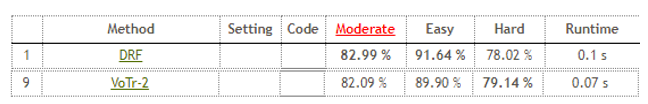
\includegraphics[scale=0.5]{Graphics/KITTI Leaderboards.png}
\caption{Current Best Results of Car Class on KITTI\cite{geiger_vision_2013} Learderboards}
\label{fig:KITTI Learderboards}
\end{figure}


\section{Motivation}
the robustness of LiDAR-based object detection model is still unknown. There may be two aspects that affect the robustness: one is adversarial attack, the other is adverse weather. Point clouds under adverse weather is point clouds, which LiDAR acquired under adverse weather, including rain, snow, fog, etc. From Figure 1.2 we could seen in the point clouds under adverse weather are significant different with clean point clouds. 
\begin{figure}[!htbp]
    \centering
    \subfigure[Clean Point Cloud\cite{geiger_vision_2013}]{
        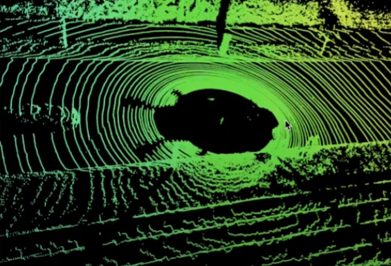
\includegraphics[width = \textwidth / 2 ]{Graphics/Clean Point Cloud.png}
        \label{fig:Clean Point Cloud}
    }
    \hspace{10pt}
     %add desired spacing between images, e. g. ~, \quad, \qquad, \hfill etc.
     %(or a blank line to force the subfigure onto a new line)
    \subfigure[Snow Point Cloud\cite{pitropov_canadian_2021}]{
        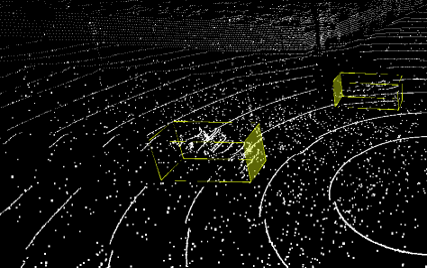
\includegraphics[width = \textwidth / 2 ]{Graphics/Snow Point Cloud.png}
        \label{fig:Snow Point Cloud}
    }
    \caption[Short Description for List of Figures]{The Differences between Clean Point Cloud and Snow Point Cloud}
    \label{fig:logo1and2}
\end{figure}
Most of the detection networks trained based on the clean point clouds may not be capable of the point clouds under adverse weather. Adversarial attack was first proposed in the field of image classification. The slight perturbation calculated with gradient is added to the original image to generate a perturbed image that is imperceptible to the naked eye, but will fool the classifier.
For point clouds detection model there's also gradient could be calculated from the loss, which could use the same method to fool the detection model.

\section{Goal Description}
For adversarial attack, slight changes to point clouds can also cause a substantial negative impact on 
the performance of detection model. For point clouds under adverse weather simulation, according to the character of point clouds under adverse weather, through adding, perturbing and dropping points methods to simulate the point clouds under adverse weather. In order for training a robust model when lack of adverse weather point clouds.
\paragraph{Contribution}
For adversarial attack there are three sections: 

the first section is FGSM. Many previous work have shown FGSM is efficient in image domain and point cloud classification domain\cite{liu_extending_2019}, this work have proved FGSM can also be applied in point cloud detection model. 

The second section is critical point drop attack. From some related studies, PointNet\cite{qi_pointnet_2017-1} defines critical points. PointPillars use a simplified PointNet to get critical features. Zheng et.al \cite{zheng_pointcloud_2019} proposed an adversarial attack by dropping critical points. By combining these thoughts, critical points in PointPillars could be defined as "critical" features in PointPillars, and execute an attack by dropping critical points. 

The first two sections are enforced on detection models.
In section three, we propose an adversarial attack method "points perturbation and points drop", it's not rely on detection model, so it can be applied in more networks. Using these methods, create benchmark datasets to test the robustness of more models. 

In the last section, simulate adverse weather point clouds to improve robustness by using additional data in adverse weather.


\section{Outline}
Introduction

Fundamentals and Related Work

Concepts

Implementations

Evaluation

Conclusion and Future work


      
% !TeX root = ../thesis.tex

\chapter{Related Works}
\label{sec:fundamentals_related-work}
In this section, we review the literature in neural network and introduce some methods of adversarial attacks.
\section{Image Object Detection Network}

Deep Neural Networks(\acrshort{dnn}) has shown highly expressive performance in the last decade and has become an indispensable tool in many practical tasks such as image classification, natural language processing and object detection. In 2012, Krizhevsky et al.\cite{krizhevsky_imagenet_2017} use a 5-layers convolutional neural network named as AlexNet achieving a considerably outstanding performance than their closest competitor \acrshort{svm}, ushering a new era in deep neural networks and encouraging further exploration in image classification. 

With the improvement of machine learning models and object representations, complete image understanding including precisely determine the class and location of the objects, known as object detection, becomes achievable and crucial. A detection work is to classify every sub-window in the image, which requires huge computational work. Two methods, region-proposal methods and end-to-end systems, are proposed to address the issues.
\subsection{Region Proposal Method}
Region-proposal method is a two-step process, taking a basic scan to suggest the promising locations and then evaluating the interest region with \acrshort{dnn} classifier. This method mainly include \acrshort{rcnn}\cite{girshick_rich_2014}, SPPNet\cite{he_spatial_2014}, Fast R-CNN\cite{girshick_fast_2015}, Faster-RCNN\cite{ren_faster_2016}, R-FCN\cite{dai_r-fcn_2016},\acrshort{fpn}\cite{lin_feature_2017}, and Mask R-CNN\cite{he_mask_2018}. 

R-CNN was proposed in 2014 by Girshick et al.\cite{girshick_rich_2014}. This network can be divided into three stages, extracting region proposals, capture features of each proposal, and classify regions with \acrshort{svm}. In the first stage, \acrshort{rcnn} takes selective search\cite{uijlings_selective_2013} to generate thousands region proposals for each image using bottom-up grouping and saliency score. Then, these chosen proposals are wrapped or cropped into a settled resolution and a 4096 dimensional feature vector is extracted by CNN as Krizhevsky proposed(ImageNet\cite{deng_imagenet_2009}). In the last step, each region proposal is scored with a trained class-specific linear \acrshort{svm}s. \acrshort{rcnn} has good performance and brings CNN into practical object detection, but both the searching and training procedures are time-consuming and storing features requires a large storage space.

Not only the speed needs to be improved, objects may also have incomplete or distort problems in the wrapping procedure. To solve these issues, He et al.\cite{he_spatial_2014} introduce spatial pyramid pooling(SPP) net, by reusing the feature maps based on the spatial positions to avoid repeated computation.

Inspired by the SPP-net, the developer of R-CNN Girshick improve his network by introducing a region of interest(\acrshort{roi}) pooling layer, which is a special case of SPP layer with only one pyramid layer\cite{girshick_fast_2015}. The training of all networks is optimized in one stage with multi-task loss on classification and bounding box regression. Fast R-CNN requires less storage space and improve the efficiency and accuracy further.

Ren et al\cite{ren_faster_2016} introduce Regional Proposal Network(\acrshort{rpn}) to replace the selective search methods. \acrshort{rpn} shares full-image convolutional layers with detection network and can predict object bounds and outputs score at each position. The proposal faster R-CNN signifies that the region proposal-based \acrshort{cnn} can be trained in end-to-end method, but the training algorithm is quite time-consuming.

Li et al.\cite{dai_r-fcn_2016} proposed region-based fully convolutional networks(R-FCN) to break down the translation invariance by inserting the \acrshort{roi} pooling layer into the convolutions manually. Compared with Faster R-CNN, the last layer of this methods outputs \(k^{2}\) position-sensitive score maps, being averaged to produce a (C+1) dimension vector, and obtain class-agnostic bounding box by adding another \(4k^{2}\) dimension convolutional layer. 

The architecture of FPN\cite{lin_feature_2017} is built with a bottom-up pathway, which downsamples the feature map and chooses the last layer output as the reference set of feature maps, a top-down pathway, where feature maps are upsampled and enhanced with same spatial size maps from bottom-up pathway, and several lateral connections. This method does not rely on CNN architectures, and can be used in object detection and other studies in computer vision, such as instance segmentation.

Instance segmentation includes two steps: detecting all the objects in the image and segmenting the instance, also known as semantic segmentation. Problems such as spurious edge or potential systematic errors on overlapping instances might occur\cite{arnab_pixelwise_2017}, and Mask R-CNN\cite{he_mask_2018} add a segmentation mask branch to solve the issues. Mask R-CNN adopts RoIAlign layer, which uses bilinear interpolation to compute the values of input features, replacing the spatial quantization for features extraction in 
\acrshort{roi} pooling. Although this improvement increases the computational volume, the substantial enhancement in accuracy and its flexibility to cooperate with other tasks make this instance-level recognition method accepted in objection detection.

\subsection{End-to-end Systems}
Different from the region proposal framework, which has multistage and each stage is trained separately, end-to-end system has only one stage using regression or classification to map image pixels straightly to bounding box. Two typical frameworks of this methods are \acrshort{yolo}\cite{redmon_you_2016} and \acrshort{ssd}\cite{liu_ssd_2016}.

Many researchers have tried to apply regression or classification to model object detection before \acrshort{yolo} and \acrshort{ssd}, but huge computing difficulty and inability to deal with overlapping objects obstruct the development. 

\acrshort{yolo}(You only look once) is a novel framework proposed by Redmon et al.\cite{redmon_you_2016}, which predict confidences and bounding boxes with the whole topmost feature map. \acrshort{yolo} consists of 24 convolutional layers and 2 fully connected layers, and it can learn priors on object positions. Additionally, decrease in false positives on backgrounds makes it possible for \acrshort{yolo} to cooperate with Fast R-CNN. Later YOLOv2, an upgrade version, adopted high resolution classifier, dimension clusters, anchor boxes etc., exhibiting expressive improvement in m\acrshort{ap} and real-time performance.\cite{redmon_yolo9000_2016}

Another end-to-end approach \acrshort{ssd}(Single Shot MultiBox Detector) was suggested by Liu et al. \cite{liu_ssd_2016}, which realizes a better balance between precision and speed. \acrshort{ssd} runs a convolutional network on the input image only once to extract a feature map, uses default anchor boxes at a variety of aspect ratios and scales, and predict bounding boxes from multiple feature maps with varied resolutions to deal with the object scale. \acrshort{ssd} realizes an outperformance than Faster R-CNN in accuracy and almost three times faster on PASCAL VOC\cite{everingham_pascal_2010} and \acrshort{coco}\cite{lin_microsoft_2015}, and more efficient than \acrshort{yolo} in dealing with large-size objects.

\section{PointCloud Classification}
3D data complement 2D images, providing shape and scale information to get a more thorough understanding of the surroundings. The representations of 3D data include point clouds, depth-maps, volumetric grids, meshes etc., and \acrshort{lidar} point clouds are used in this paper. 

Point clouds can be classified as Multiview-based, point-based and voxel-based methods. Multiview based methods firstly project point clouds into multiple views, extract and fuse features for classification. 

Su et al.\cite{su_multi-view_2015} introduce MVCNN, which is a pioneer work, proving that combining multiple views of a 3D shape information into a compact descriptor could attain a good recognition performance. The procedure of aggregating multi-view features to global shape descriptor is the main challenge of this approach, which inspires researchers to exploit progressive feature aggregation strategy. 

One attempt of Wei and his colleagues \cite{wei_view-gcn_2020} is to regard multiple views as graph nodes and construct a hierarchical graph \acrshort{cnn} to learn global shape descriptor. They name the network as view-GCN, which achieves high accuracy in point cloud classification and retrieval and outperform other methods on RGB-D dataset\cite{lai_large-scale_nodate}.

Voxel-based method, also known as volumetric-based method, is to voxelize a point cloud into 3D grids and classify the point cloud by introducing volumetric representation on CNN training. With the proposal of VoxNet\cite{maturana_voxnet_2015} by Maturana, the idea of transforming a 3D model into an occupancy grid is widely accepted and encourages promotion of the VoxNet and its variants. 

Wu et al\cite{wu_3d_2015} propose to use a binary probability distribution on a voxel grid to demonstrate a geometric 3D shape, applying on convolutional deep belief network. The recognition accuracy is impressive on various recognition tasks and on different datasets, but the ability to scale dense 3D data is limited due to the large computational and storage requirements. 

To better represent the point clouds geometry information, PointGrid was introduced by Le et al.\cite{le_pointgrid_2018}, which is \acrshort{cnn} integrated point and grid. The network is embedded a regular-structured volumetric grid to hierarchically extract global information and incorporates constant points number within each grid cell to overcome the limitation of grid cell. Compared with existing state-of-art methods, this approach has advantages in speed and memory requirements.
  
Methods based on multiple view images and voxel grids all adopt the views from image neural network, different from them, point-based approach works on raw point clouds directly, simplifying the process and reducing the information loss during projection or voxelization. In terms of network architecture, point-based method can be categorized into convolution-based, graph-based, pointwise \acrshort{mlp} and other methods. 

Considering the irregularity of point data, point-wise \acrshort{mlp} methods use Multi-Layer Perceptron to process each point independently, then use a symmetric aggregation function to derive a global feature. An innovative and simple network PointNet\cite{qi_pointnet_2017} directly takes point clouds as input and treat these input points independently and identically. Max pooling layer uses a single symmetric function, respecting the permutation invariance, to select informative points in the point cloud, which is the key part of PointNet. In the final step, the network aggregate learnt information to the global descriptor for further point cloud classification and segmentation. PointNet exhibits strong stability and efficiency empirically and the ideas are transferred and advanced in further research.

Incapability to capture local structures of PointNet motivates Qi et al.\cite{qiPointNetDeepHierarchical2017} to put forward an improved version, PointNet++. This hierarchical network partitions point sets into local regions according to the metric space distance firstly, then further group local features to capture high-level representations until collect the features of the whole point set. Unlike the single max pooling layer, PointNet++ involves a number of set abstraction levels, which is made of sampling layer, grouping layer and PointNet layer. By abstracting increasingly broader local regions along the hierarchy, PointNet++ is able to capture local features with increasingly larger scales, and the efficiency and robustness are both proved significantly better than other benchmarks in point clouds study.

\section{\acrshort{lidar}-based Object Detection Network}
The availability and reliability of 3D sensors such as \acrshort{lidar}, RGB-D camera and various 3D scanners, make it possible for autonomous vehicles equipped with multiple sensors collect more accurate and detailed information. The input of 3D object detector is the point clouds of a scene and a 3D bounding box is sketched around the detected target. The approaches of 3D object detection are divided into two types: region proposal methods and single shot methods. 
\subsection{Region Proposal-based Methods}
Adopting the idea in 2D image object detection, region proposal-based methods in 3D object detection consists of three categories regarding to the means of generating object proposal, specifically Multiview-based, segmentation-based and frustum-based, and the representative networks of which are shown in Figure \(\ref{fig:LiDAR Region Proposal}\)
\subsubsection{Multi-view based Methods}
The general idea of Multiview methods is integrating proposal-wise features from various point cloud projections, such as \acrshort{lidar} front view and \acrshort{bev} (Bird’s Eye View), to generate 3D rotated boxes. The specific process is shown in Figure\(\ref{fig:LiDAR Region Proposal}\) (a). MV3D, a sensory-fusion framework, is proposed by Chen et al.\cite{chen_multi-view_2017} Taking \acrshort{lidar} point cloud and RGB images as the input to generate oriented 3D bounding boxes. The network consists of two subnetworks, to generate 3D object proposals and to fuse multi-view features respectively. 3D candidate boxes are generated in the first subnetwork from the \acrshort{bev} map projected by 3D point clouds, and region-wise features from multiple views are combined in the deep fusion scheme in the second subnetwork. MV3D achieves higher AP in 3D localization and detection than current state-of-the-art methods.

To improve fusion efficiency in Multiview-based methods, Ku et al \cite{ku_joint_2018} proposed AVOD (aggregate view object detection) network including a region proposal network and a second stage detector network. A novel architecture, is introduced in the \acrshort{rpn} step, which can perform multi-modal feature fusion to produce region proposals for small objects with a high recall. 

\subsubsection{Segmentation-based Methods}
Achieving higher recall rates and outperformance in complexed scenes than Multiview-based methods, segmentation-based methods remove most background points with the semantic segmentation techniques and then generate plentiful high-quality points on foreground points. Shi et al. \cite{shi_pointrcnn_2019} come up with the PointRCNN, which generates proposals by segmenting point clouds directly into foreground objects and refines proposals by combining local spatial features and semantic features. The process is shown in Figure \(\ref{fig:LiDAR Region Proposal}\) (b),

A sequential fusion method, PointPainting was proposed by Sourabh et al.\cite{vora_pointpainting_2020}, which is a flexible framework that has three stages: semantic segmentation, fusion, and object detection. In the semantic segmentation network, pixel-wise segmentation scores are computed and served as compact image features, and then points are painted with the scores and fed into detectors. On the KITTI benchmark, PointPainting offering a fast, accurate and robust results in extensive experimentation.

\subsubsection{Frustum-based Methods}
Qi et al., the constructor of PointNet, contributed a pioneering work using frustum-based method, called F-PointNets\cite{qi_frustum_2018}. The procedure is shown in Figure \(\ref{fig:LiDAR Region Proposal}\) (c), which extracts 3D frustum proposals from 2D candidate regions generated by image object detectors firstly, then carry out instance segmentation to predict the 3D mask of the target object, and lastly perform regression using PointNet variants to estimate a modal 3D bounding box. By leveraging both 2D detectors and 3D \acrshort{dl} techniques for object localization, this model is able to provide accurate 3D bounding boxes under situations of occlusion or partial data. 

\begin{figure}[!htbp]
\centering
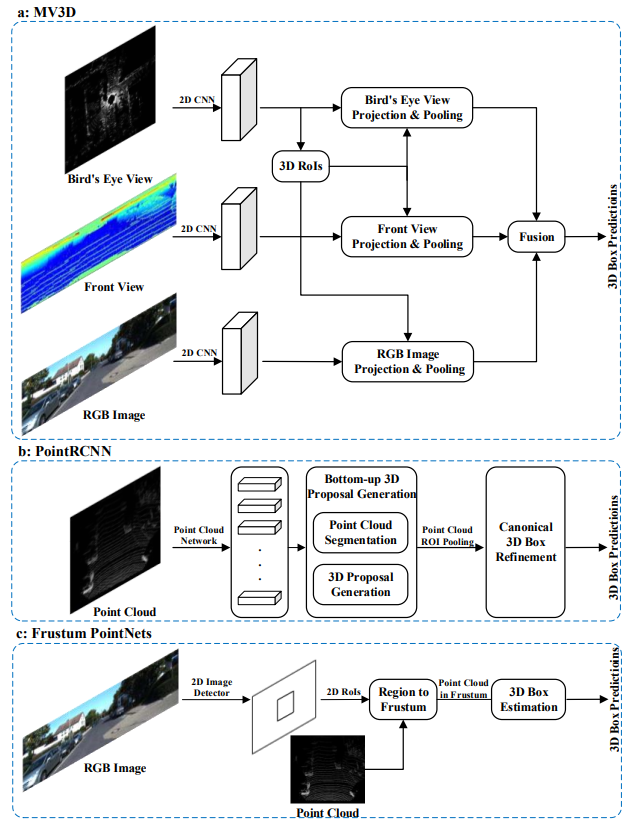
\includegraphics[scale=0.7]{Graphics/LiDAR Region Proposal.png}
\caption{Typical networks for three categories of region proposal-based 3D object detection methods.\cite{guo_deep_2020} From top to bottom: (a) multi-view based, (b) segmentation-based and (c) frustum-based methods.}
\label{fig:LiDAR Region Proposal}
\end{figure}

\subsubsection{Other Methods}
By deeply intergrating 3D voxel \acrshort{cnn} and PointNet-based set abstraction, a recent unified 3D object detection framework PointVoxel-RCNN was introduced by Shi et al.\cite{shi_pv-rcnn_2021}. It is a two-stage strategy, specifically voxel-to-keypoint and keypoint-to-grid. In the first step, voxel-based CNN is adopted to learn voxel-wise multiscale features and generate accurate 3D proposals, and then voxel-wise features are groupped to aggregate key point features via PointNet-based set abstraction. In the second stage,  a ROI-grid pooling module incorporated with key point features is established to learn proposal features for subsequent proposals refinement and confidence prediction. The empirical results demonstrate outstanding performance with high ranking on KITTI dataset and Waymo Open dataset\cite{sun_scalability_2020}.
Shi et al.\cite{shi_pv-rcnn_2021} proposed PointVoxel-RCNN (PV-RCNN) to leverage both 3D convolutional network and PointNet-based set abstraction for the learning of point cloud features. Specifically, the input point clouds are first voxelized and then fed into a 3D sparse convolutional network to generate high-quality proposals. The learned voxel-wise features are then encoded into a small set of key points via a voxel set abstraction module. In addition, they also proposed a keypoint-to-grid \acrshort{roi} abstraction module to capture rich context information for box refinement. Experimental results show that this method outperforms previous methods by remarkable margin. 

To improve the preliminary work PointRCNN from the inspiration of 3D ground-truth boxes, Shi et al proposed a Part-\(A^{2}\) net\cite{shi_points_2020}, which is composed of two stages: part-aware stage and part-aggregation stage. The part-aware stage utilizes accurate intra-object parts locations provided by ground truth boxes and groups the intra-object information via \acrshort{roi}-aware point cloud pooling module. Then in the part-aggregation stage, spatial relationship of the pooled intra-object info are used to refine the box location. This method introduces intra-object part locations learning for the first time and effectively enhance the 3D object detection performance.

\subsection{Single Shot Methods}
Extending the end-to-end approach in image to 3D object detection, single shot method is a single-stage network that can predict class probability and regress 3D bounding boxes directly. Zhou and Tuzel\cite{zhou_voxelnet_2017} introduce VoxelNet, which merges the feature extraction and bounding box generation into one stage. VoxelNet partitions point cloud into equally spaced voxels firstly, and transforms points in each voxel into features via \acrshort{vfe} layer, resulting in a volumetric representation of points clouds, which can cooperate with \acrshort{rpn} for further detection work. The performance of VoxelNet is strong, but the large computational cost and low speed constrain its feasibility in real-time applications. 
\subsubsection{Discretization-based Methods}
Adopting the voxel-based feature extraction method, Yan et al.\cite{graham_3d_2017} put forward a novel approach aiming to increase the speed and orientation estimation performance\cite{yan_second_2018}. Following the voxel feature extractor, a spatially sparse convolution is used to extract feature from z-axis before generating \acrshort{bev} images, and GPU-based generation algorithm are used for sparse convolution to enhance the speed further. Considering the large loss caused by the difference in orientation between ground truth and prediction when their bounding boxes are overlapping, an innovative angle loss regression is proposed to improve performance. A data augmentation approach based on capacity is introduced which exhibits substantial enhancement in convergence speed and performance.

A new encoder PointPillars, proposed by Lang et al.\cite{lang_pointpillars_2019}, transforms point clouds to pillars and utilizes PointNets to extract features on pillars. The network incorporates three stages: a encoder learn features and scatter back the learned features to a pseudo image, a backbone of 2D convolution convert the pseudo-image into a concatenation of all feature maps, and use \acrshort{ssd} methods to predict 3D bounding boxes in the last step. From the experimental results on the KITTI\cite{geiger_vision_2013} dataset, PointPillars shows dominant outperformance in AP at a higher speed, comparing with other existing methods.

\section{Adversarial Attacks and Defenses}
Evolved from back-propagation algorithm, gradient-based attacks make a slight modification to develop a perturbation vector for the input. Keeping the model weights constant and considering the input as a variable, gradients of each input element can be obtained and can be utilized to generate perturbation vector. Some widely used adversarial attack techniques include FGSM\cite{goodfellow_explaining_2015}, BIM(Iterative-FGSM\cite{kurakin_adversarial_2017}), FGSM with momentum\cite{dong_boosting_2018}, PGD\cite{madry_towards_2019} etc.

FGSM(Fast gradient sign method) ,proposed by Goodfellow et al.\cite{goodfellow_explaining_2015} is the main approach used in this paper. The general idea is to generate adversarial examples with the use of the gradient of the loss function with respect to an upper bound of the perturbation. The gradient of the loss function can be computed in deep neural networks in a fast speed, so it is named FGSM. This method is widely accepted in 2D image object detection tasks\cite{liu_detection_2018,kurakin_adversarial_2017}, also provides insight in 3D point clouds attack\cite{zeng_adversarial_2019}. More specific explanation of loss function and description of FGSM variants will be displayed in the next section.

Jacobian-based Saliency Map Attack (JSMA) is a practical gradient-based attack method relies on Jacobian matrix, is firstly proposed in image classification work by Papernot et al.\cite{papernot_limitations_2015}. It’s a forward derivative matrix used to build adversarial saliency maps, incorporating a specific perturbation in the input features to generate adversarial samples. This method achieves 97\% adversarial success rate with modification on average 4.02\% input features in each sample. JSMA is applicable to control adversaries with respect to the perturbation choice based on the adversarial goals. Some variants of JSMA grant this method more flexibility, M-JSMA lower the requirements of specifying the target class and the direction of perturbation, but still provides competitive speed and performance\cite{wiyatno_maximal_2018}, Weighted-JSMA utilizes the output probabilities to apply a weighting on the saliency map, showing the faster and more efficient non-targeted attacks than JSMA. Based on WJSMA, Taylor-JSMA take additional step to penalize external input features, giving better performance in target attack than WJSMA\cite{wiyatno_maximal_2018}.

Besides attacks in images, JSMA method can also be extended to attacking point clouds classifiers. Liu et al.\cite{liu_extending_2019} modified the JSMA slightly by considering gradients of three dimensions of the point and add perturbations in all three dimensions. Depending on the gradients, the value of dimensions can be changed, leading to the increase of candidate points to be perturbed. However, the attack effectiveness of JSMA is not satisfying with a lower success rate empirically compared with other FGSM and FGSM variants.

Defense is the operation to train neural network to make the attacks fail as much as possible. Papernot et al.\cite{papernot_distillation_2016} suggest a defensive mechanism named defensive distillation, to train DNN classifier to be more robust to perturbation. First step is to train a network on the training data with a softmax temperature, then use a probability vector which has additional class probabilities knowledge to train a distilled network at the same temperature and same training data. The empirical results on the MNIST dataset indicates resilience increase of DNNS to adversaries and improve class generalizability.

Defense on JSMA and its variants are investigated in(Probabilistic Jacobian-based Saliency Maps Attacks). By adding adversarial samples produced by JSMA, WJSMA, TJSMA to the training set, networks against TJSMA and WJSMA provide the better performance than JSMA from the view of defender.

Applied the optimization method to craft adversarial samples, Carlini and Wagner\cite{carlini_towards_2017} construct three powerful attacks \(L_{0},L_{1},L_{\infty}\), which can defeat the defensive distillation(distillation as a defense to adversarial perturbations against deep neural networks), providing a better baseline for evaluating the efficacy defenses model. They generate adversarial examples by iteratively minimize the distance metric between real and adversarial image under different constraints. CW attacks perform well in terms of success rate on IMAGENET dataset\cite{carlini_towards_2017,rottmann_detection_2021}, but it shows high computational cost and less convenient in the real-time applications\cite{combey_probabilistic_2020}. C\&W attack approach illuminates further adversarial attack approach such as EAD\cite{chen_ead_2018},\cite{sharif_accessorize_2016},()

DeepFool is another optimization-based method, proposed by Moosavi-Dezfooli et al.\cite{moosavi-dezfooli_deepfool_2016}. This method suggests an iterative linearization algorithm DeepFool, which can effectively compute adversarial perturbations and accurately evaluate the robustness of classifiers in a high speed, expecting to be a baseline method on large-scale datasets.

Xiao et al.\cite{xiao_generating_2019} were the first to utilize generative adversarial networks(GANs) to produce adversarial samples.  Applying to black-box attack and semi-white box attack, AdvGAN achieves high attack success rate and exhibits resilient under existing defenses. Besides, unrestricted adversarial examples trained on AG-GAN\cite{odena_conditional_2017} was introduced by Song et al.\cite{song_constructing_2018}. Specifically, the adversarial examples are generated from scratch using conditional generative models rather than perturbing existing points, providing an instructive and innovative view to construct adversarial examples. Simultaneously, GAN-based approaches has been attracting growing interests recently and a promising future is approaching.

Inspired by C\&W approach, Xiang et al.\cite{xiang_generating_2019} make an attempt to craft adversarial samples of 3D point clouds and propose a novel algorithm against PointNet\cite{qi_pointnet_2017} and create adversarial examples in two perspectives. One is adversarial point perturbation, by negligibly shifting existing points, another is adversarial point generation, by placing sets of scattered and independent points or some point clusters similar to the original object.After extensive experiment with ModelNet40 dataset, very high success rates (over 99\%) are demonstrated for six designed attacks under different perturbation metrics, providing a guideline for further 3D adversarial samples design. Optimization attack algorithms are vigorously promoting creative techniques in crafting 3D adversarial samples, such as in \cite{wicker_robustness_2019,athalye_synthesizing_2018}

Yang et al.\cite{yang_adversarial_2019} propose a skeleton-detach attack method on point clouds, which enhance the speed than previous gradient-based and optimization-based attacks. The method is conducted by detaching the most critical points from the critical subset referred in PointNet iteratively. Tansferability of attacks between different networks, an unsettled problem in the method of Xiang et al.\cite{xiang_generating_2019}, is successfully solved in this approach, but the success rate is declined compared with previous works.

To overcome the hindrance of speed exposed in gradient-based and optimization-based method, and flexibility limitation in skeleton detach methods\cite{yang_adversarial_2019}, Zhou et al.\cite{zhou_lg-gan_nodate} introduce a faster and flexible method label guided adversarial network(LG-GAN) to attack 3D point clouds. The general process is as follows, LG-GAN leverages an adversarial network to extract the features of input point clouds, then use the label encoder to merge specified label information into features, the last step is to feed the encoded features into the decoder to produce adversarial samples. By attacking point cloud network such as PointNet, PointNet++ and DGCNN along with other existing attack methods, Zhou et al. prove that LG-GAN outperforms FGSM and IFGSM in both speed and success rate, and reaches a similar performance as C\&W method with substantially higher speed.

Aiming at generating adversarial attacks on 3D point clouds with transferability of networks, Hamdi et al develop dubbed AdvPC\cite{vedaldi_advpc_2020}, in which the attack is generated with an accessible victim network and the adversarial sample can be applied to an inaccessible and unseen transfer network. An auto-encoder(AE), which can reconstruct the perturbed input, is introduced in the method to generate more transferable attacks. Through multiple tests on point clouds network such as PointNet, PointNet++, DGSNN, high attack success rate and better transferability than other existing 3D attacks are provided. Additionally, Hamdi et al also demonstrate that compared to other baselines on the ModelNet40, AdvPC can increase the ability to break defenses by approximately 40\%.

Denoiser and Upsampler Network(DUP-Net\cite{zhou_dup-net_2019}), proposed by Zhou et al, is a defense approach for adversarial attacks on 3D point cloud classification. This network is merge of SOR(statistical outlier removal\cite{rusu_towards_2008}) layer and PU-Net\cite{li_pu-gan_nodate}, presenting that additional robustness is offered by removing statistical outliers and the upsampler network can defend well against adversarial attacks such as \acrshort{cw} attacks.
     
% !TeX root = ../thesis.tex

\chapter{Concepts}
\label{sec:concepts}





 \section{Adjustment after Perturbed Points}
 
 LiDAR points have different azimuth and elevator, which are two angles represents emitter angle of the points. The differences of two angles between points from adjacent emitter should be the same. When the perturbed point is green point, it have the same two angles as the original point. If perturbed point goes to red point, then the perturbed point's two angles should be adjusted to the original degrees, in order for keeping the physical character of LiDAR point clouds.
 \begin{figure}[!htbp]
\centering
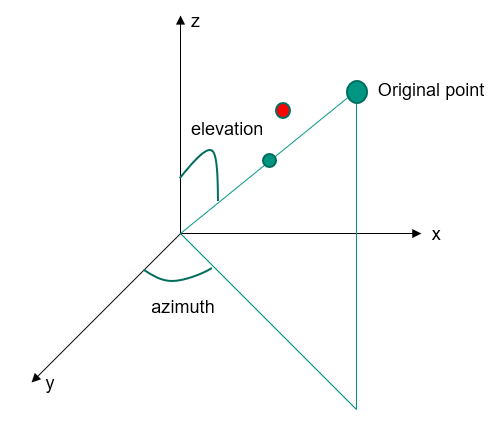
\includegraphics[scale=0.5]{Graphics/Adjustment.png}
\caption{LiDAR Point Coordinate System}
\label{fig:Adjustment}
\end{figure}

\section{Drop Critical Points}

\begin{enumerate}
 \item \textit{Critical Features}
 
PointPillars\cite{lang_pointpillars_2019} uses simplified PointNet\cite{qi_pointnet_2017}, which is called Pillar Feature Net. Pillar Feature Net's first two step is import for definition of critical features. The first step is to stack points into pillars, the second step is to get learned features in each pillar. The learned features is defined as critical features.
\begin{figure}[!htbp]
\centering
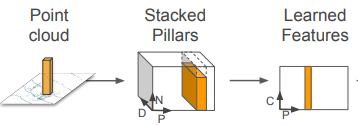
\includegraphics[scale=1]{Graphics/Pillar Feature Net.png}
\caption{Part of Pillar Feature Net}
\label{fig:Pillar Feature Net}
\end{figure}
\item \textit{Critical Points}

Definition critical points with two criterion:

1. Critical point in each pillar is the point with maximum critical feature value. 

2. Critical point is the point that has most critical features.

In Figure 4.4, cells with critical features are pinpointed in colored background. In the whole table, 10 is the maximal critical feature value, and it's located at the third row, so this point is a critical point from first criterion. When counting the number of critical features, the fourth row has four colored cells, showing it has most features than other points. So, this point is a critical point based on second criterion.
\begin{figure}[!htbp]
\centering
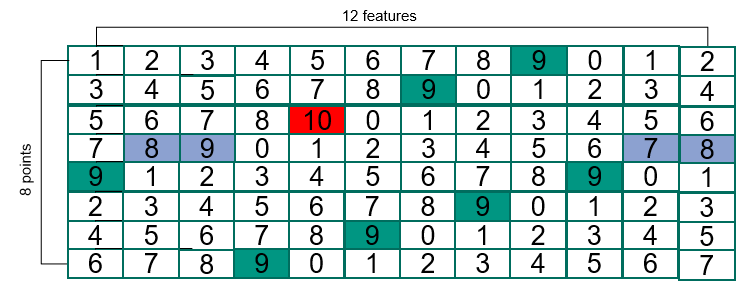
\includegraphics[scale=0.5]{Graphics/Critical Points.png}
\caption{Pseudo Process of Catching Critical Features}
\label{fig:Critical Points}
\end{figure}
\end{enumerate}

\section{Points Perturbation and Points Drop}

\begin{enumerate}
\item\textit{Points Perturbation and Points Drop methods}

1. Points Perturbation on different features: intensity \(r\), \(xyz\) coordinates, and the combination of \(xyz\) coordinates and intensity \(r\).
2. Points randomly drop: the number of dropping points rely on the total number of points.
 \item \textit{Benchmark}
 To evaluate the robustness, rPC, which is the relative performance under point cloud changes, is used. RPC is the ratio of mPP and \(P_{clean}\):
\begin{center}
          \(rPC = \frac{mPC}{AP_{clean}} \)
\end{center}
\(AP_{clean}\) is the average precision of the detection model under clean dataset, and mPC is the mean value of average precision of detection under benchmark datasets:
\begin{center}
          \(mPC = \frac{1}{N_{C}}\sum_{c=1}^{N_{C}}\sum_{s=1}^{N_{S}}{AP_{C,S}} \)
\end{center}
\({P_{C,S}}\): performance evaluated on data changed with changes C with perturbation and drop points under severity level S

\({N_{C}}\): number of changes, including different methods

\({N_{S}}\) :severity levels

\end{enumerate}

\section{Adverse Weather Point Clouds Simulation}

\begin{enumerate}
 \item \textit{Simulate Methods}
 
 1. Add gaussian noise perturbation.

2. Drop points randomly.

3. Add points surround cluster and ground points. Use RANSAC to segement ground points of lidar point clouds and then get clusters with DBSCAN. Random pick the some points in cluster and ground points to do the gaussian noise perturbation and then add the perturbated points to the original points as the addition of noise points.
 
 \item \textit{Evaluation Metric: Weather Classification} 
 
 Vargas et.al\cite{vargas_rivero_weather_2020} have shown, use simple statistic parameters of point clouds: standard deviation and mean value of \(x\) coordinates and mean and standard deviation of echo-pulse width, which is intensity, etc. 13 parameters as input for a weather classifier.
 \item \textit{Evaluation Metric: Weather Points Semantic Segmentation}
 
 
 Evaluate the performance of simulation, weather point semantic segementation network is introduced. As the figure 6 shown, the DENSE Dataset labeled each point cloud with a weather category, which is adverse weather consists of rain and fog. Heinzler et.al \cite{heinzler_cnn-based_2020} proposed WeatherNet training on DENSE Dataset. His results is shown in Table 4.1
 \begin{table}[h!]
  \begin{center}
    \caption{Training Results on DENSE Dataset}
    \begin{tabular}{|c|c|c|c|} % <-- Alignments: 1st column left, 2nd middle and 3rd right, with vertical lines in between
      \hline
      \multirow{2}{*}{Methods} & \multicolumn{3}{c|}{Weather Class}\\
    \cline{2-4}
       &\textbf{Clean(mIOU)} & \textbf{Rain(mIOU)}& \textbf{Fog(mIOU)}\\
      \hline
      WeatherNet & 93.35 & 90.92&88.81\\
      Cylinder3D & 98.91 & 94.61&91.63\\
      \color{blue}
      Delta & \color{blue}+5.56 & \color{blue}+3.69&\color{blue}+2.28\\
    \hline
    \end{tabular}
  \end{center}
\end{table}
Cylinder3D\cite{zhu_cylindrical_2020} performs well in Semantic KITTI\cite{behley_semantickitti_2019}, which is an object semantic datasets. 
\end{enumerate}

% !TeX root = ../thesis.tex

\chapter{Implementation}
\label{sec:implementation}



% !TeX root = ../thesis.tex

\chapter{Evaluation}
\label{sec:evaluation}

\sisetup{round-mode = places, round-precision = 2, scientific-notation = fixed, fixed-exponent = 0}
\begin{table}[!htbp]
    \centering
    \begin{tabular}{crSSSSSS}
        \hline
        & & \textbf{mean} & \textbf{median} & \textbf{stddev} & \textbf{min} & \textbf{max} & \textbf{other}\\%
        \hline
        \parbox[t]{2mm}{\multirow{3}{*}{\rotatebox[origin=c]{90}{Data1}}}
        & Lane 1 [m] & 3.78e+00 & 3.78e+00 & 8.06e-02 & 3.58e+00 & 4.23e+00 & 3.75\\
        & Lane 2 [m] & 3.84e+00 & 3.84e+00 & 4.58e-02 & 3.58e+00 & 4.02e+00 & 3.75\\
        & Lane 3 [m] & 3.82e+00 & 3.81e+00 & 8.30e-02 & 3.31e+00 & 4.06e+00 & 3.75\\
        \hline
    \end{tabular}
    \caption[Short Description for List of Tables]{
      Long Description for under the table.
    }\label{tab:xy}
\end{table}

\blindtext

% !TeX root = ../thesis.tex

\chapter{Conclusion and Future Work}
\label{sec:conclusion_future-work}

\section{Conclusion}
FGSM and critical point drop prove that LiDAR-based detection model are vulnerable to adversarial attack. FGSM defense confirms that adversarial training of LiDAR-based detection model can defense adversarial attack. Points perturbation and points drop datasets provide a benchmark dataset to benchmark robustness of LiDAR-based detection models. Adverse weather points simulation improves robustness by using additional data in adverse weather.

\section{Future Work}
In simulation of adverse weather point cloud, we could use more realistic simulation by adding perturbation of clusters and ground points.
      

%% --------------------
%% |   Appendix+Verzeichnisse   |
%% --------------------
\appendix
\chapter{Appendix}
\label{appendix}

\section{Acronyms and Notations}
\label{sec:eval_param}

\newpage
%--------------------------------------------------------------------------------


% List of Figures
\cleardoublepage
\addcontentsline{toc}{chapter}{\listfigurename}
\listoffigures

% Liste of Tables
\cleardoublepage
\addcontentsline{toc}{chapter}{\listtablename}
\listoftables

% Bibliography
\bibliographystyle{IEEEtranSA}   		% IEEE Alphanumeric
\cleardoublepage
\addcontentsline{toc}{chapter}{Bibliography}
\bibliography{references}
% Online References
\ifuseglossaries
	\printglossary[type=onlineref, style=mylist]
\else
\fi

\end{document}
